\documentclass{jlreq}

\usepackage{amsmath}
\usepackage{bm}
\usepackage{fancyhdr}
\usepackage{float}
\usepackage{graphicx}
\usepackage{physics}
\usepackage{siunitx}

\numberwithin{equation}{section}

\pagestyle{fancy}
\fancyhf{}
\fancyhead[R]{\thepage}

\begin{document}

\tableofcontents
\clearpage

\section{目的}
% 「ミュラーリヤー錯視」図形を例として,刺激条件と認知との間の法則性を理解するとともに,認知
% 特性に関する実験方法,分析方法を学ぶ.
ミュラーリヤー錯視の実験を行い,矢羽の角度が同じ場合に上昇系列と下降系列で測定で錯視量に相違があるのかどうかの分析を行い,矢羽の角度と錯視量の関係性について考察を行う.
また,認知特性に関する実験方法と分析方法を身に着ける.

\section{実験機材}
使用した機材は,Dell\ Inspiron\ 15\ 3535である.OSはWindows11\ Homeであり,用いたR言語はR\ version\ 4.3.2である.
また,配布物は$3\si{\cm}$の矢羽と$10\si{\cm}$の主線が印刷された,鋏角が$60\si{\degree}, 120\si{\degree}, 180\si{\degree}, 240\si{\degree}, 300\si{\degree}$の5種類の標準刺激と,線とスケールが印刷された比較刺激である.
標準刺激の例を図\ref{fig:std_stim}に示す.

\begin{figure}[H]
  \centering
  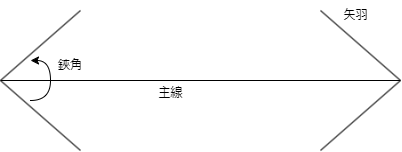
\includegraphics[width=0.5\textwidth]{image/ミュラーリヤー錯視.png}
  \caption{標準刺激の例}
  \label{fig:std_stim}
\end{figure}

\section{実験方法}
\subsection{ミュラーリヤー錯視に関する測定}
まず,5種類の標準刺激を比較刺激に差し込みスライドすることで比較刺激を調整して,標準刺激の主線と等しい長さに見える比較刺激の直線の長さ(主観的等価点, point\ of\ subjective\ equality:PSE)を求めた.
測定の際,比較刺激が最も短く見える地点から調整を開始する上昇系列と,比較刺激が最も長く見える地点から調整を開始する下降系列について,それぞれ4回ずつ測定を行った.
得られた測定結果を,2つの系列について平均を求め,基準値10から引くことで錯視量を求め,2班のデータを表計算ソフトにまとめた.

\subsection{測定結果の統計分析}
班のデータを用いて,5種類の刺激条件毎にt検定を行い,上昇系列と下降系列の錯視量の平均値を比較した.次に,上昇系列と下降系列を別にして,
5種類の刺激条件間の錯視量の平均値の比較を分散分析により行った.

\section{結果}
個人のPSE測定の結果を図\ref{fig:myPSE}に示す.なお,本実験では上昇系列をA,下降系列をDと表現している.

\begin{figure}[H]
  \centering
  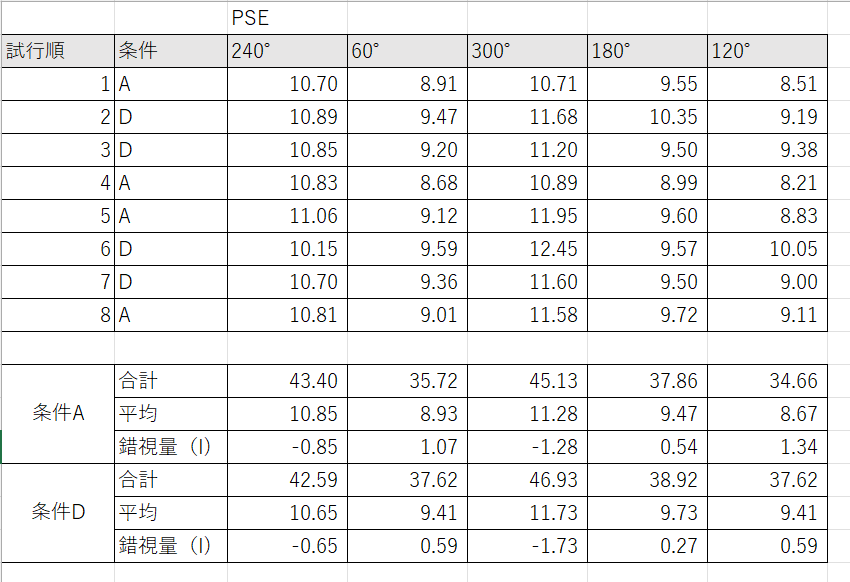
\includegraphics[width=0.8\textwidth]{image/myPSE.png}
  \caption{実験者個人の錯視量の測定結果}
  \label{fig:myPSE}
\end{figure}

班員の刺激条件毎の錯視量のデータを図\ref{fig:group_data}に示す.また,有意水準を$5\si{\percent}$として統計分析を行った.
\begin{figure}[H]
  \centering
  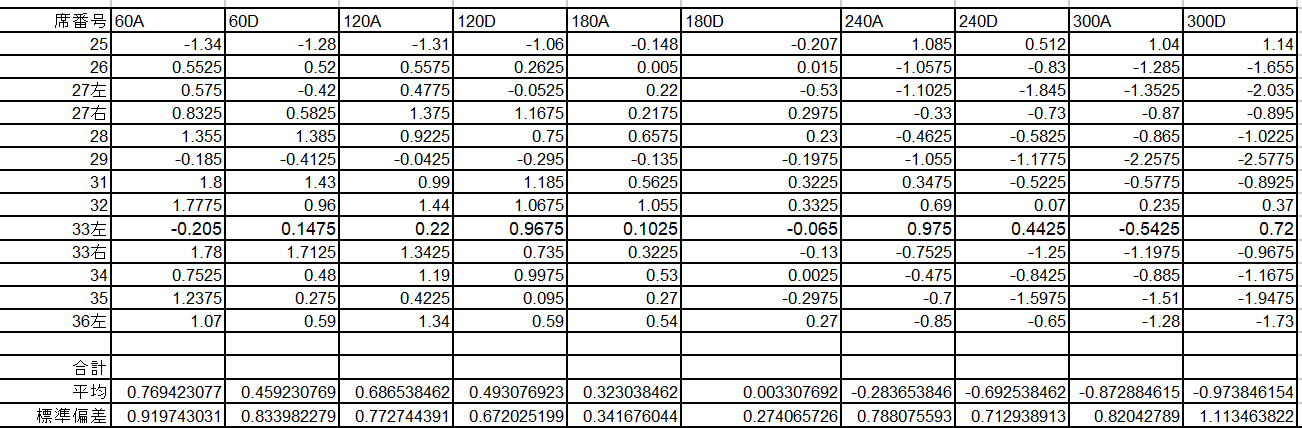
\includegraphics[width=\textwidth]{image/錯視量_班員データ.png}
  \caption{刺激条件毎の錯視量のデータ}
  \label{fig:group_data}
\end{figure}

\subsection{上昇系列と下降系列の錯視量の比較}
鋏角が$60\si{\degree}, 120\si{\degree}, 180\si{\degree}, 240\si{\degree}, 300\si{\degree}$の5種類の標準刺激毎に,系列Aと系列Dの錯視量の平均値を対応のあるt検定により比較した結果を
鋏角の昇順に図\ref{fig:60degree}-図\ref{fig:300degree}に示す.

\begin{figure}[H]
  \centering
  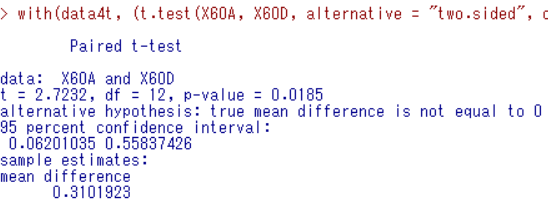
\includegraphics{image/60degree.png}
  \caption{鋏角が$60\si{\degree}$のときの,t検定の結果}
  \label{fig:60degree}
\end{figure}

\begin{figure}[H]
  \centering
  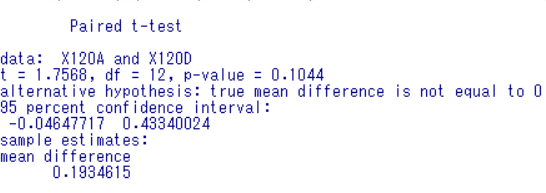
\includegraphics{image/120degree.png}
  \caption{鋏角が$120\si{\degree}$のときの,t検定の結果}
  \label{fig:120degree}
\end{figure}

\begin{figure}[H]
  \centering
  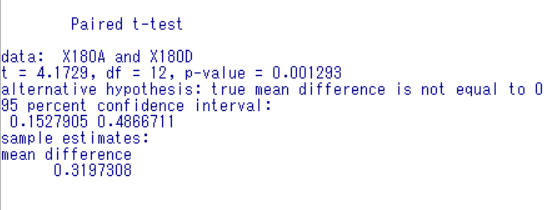
\includegraphics{image/180degree.png}
  \caption{鋏角が$180\si{\degree}$のときの,t検定の結果}
  \label{fig:180degree}
\end{figure}

\begin{figure}[H]
  \centering
  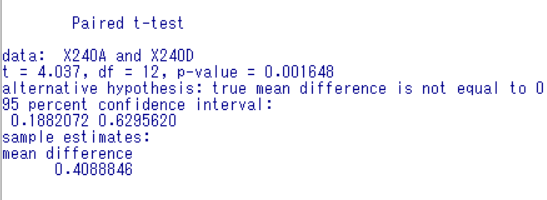
\includegraphics{image/240degree.png}
  \caption{鋏角が$240\si{\degree}$のときの,t検定の結果}
  \label{fig:240degree}
\end{figure}

\begin{figure}[H]
  \centering
  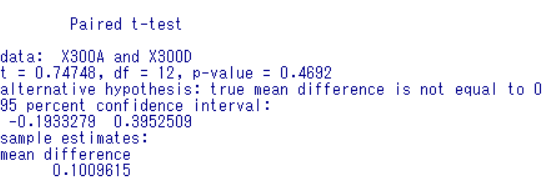
\includegraphics{image/300degree.png}
  \caption{鋏角が$300\si{\degree}$のときの,t検定の結果}
  \label{fig:300degree}
\end{figure}

\subsection{矢羽の角度と錯視量の関係についての実験}
2つの系列A,Dそれぞれに対して,分散分析を行った結果を図\ref{fig:about_A_oneway}-図\ref{fig:about_D_multi}に示す.

\begin{figure}[H]
  \centering
  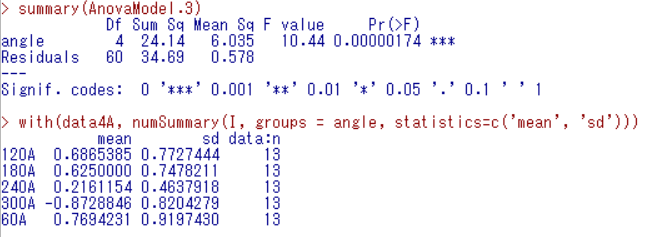
\includegraphics{image/about_A(一元).png}
  \caption{系列Aに対する,一元配置分散分析の結果}
  \label{fig:about_A_oneway}
\end{figure}

\begin{figure}[H]
  \centering
  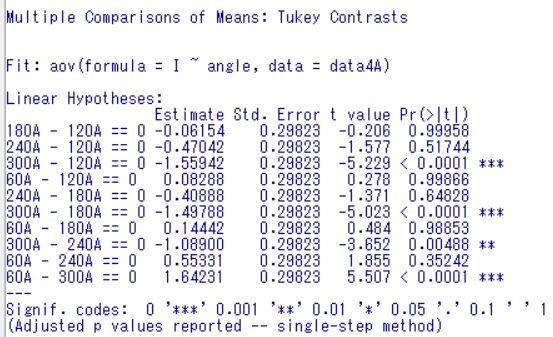
\includegraphics{image/about_A(多重).png}
  \caption{系列Aに対する,多重比較の結果}
  \label{fig:about_A_multi}
\end{figure}

\begin{figure}[H]
  \centering
  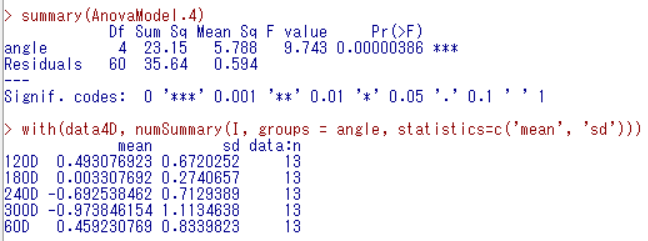
\includegraphics{image/about_D(一元).png}
  \caption{系列Dに対する,一元配置分散分析の結果}
  \label{fig:about_D_oneway}
\end{figure}

\begin{figure}[H]
  \centering
  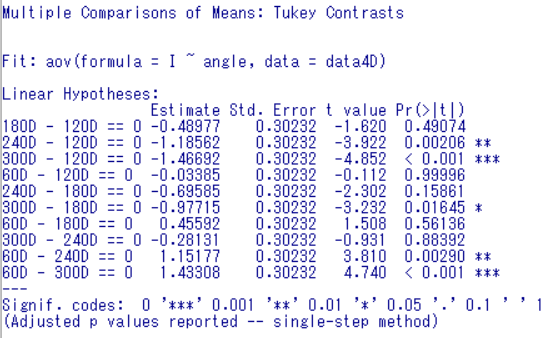
\includegraphics{image/about_D(多重).png}
  \caption{系列Dに対する,多重比較の結果}
  \label{fig:about_D_multi}
\end{figure}

また,系列Aと系列Dの分散分析結果のグラフを図\ref{fig:result_a},図\ref{fig:result_d}に示す.
\begin{figure}[H]
  \centering
  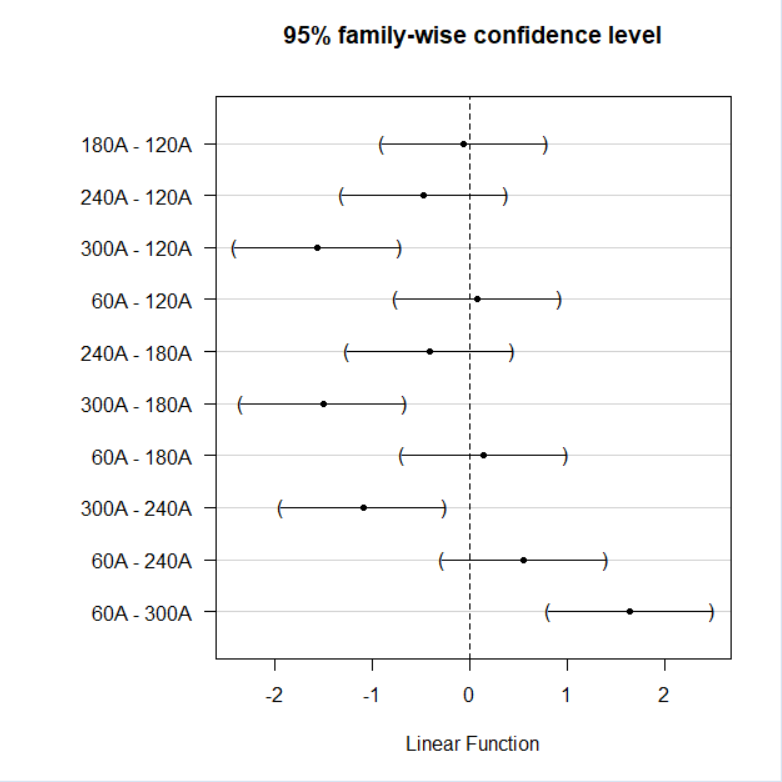
\includegraphics[width=0.6\textwidth]{image/a_信頼区間.png}
  \caption{上昇系列(A)の分散分析の結果}
  \label{fig:result_a}
\end{figure}

\begin{figure}[H]
  \centering
  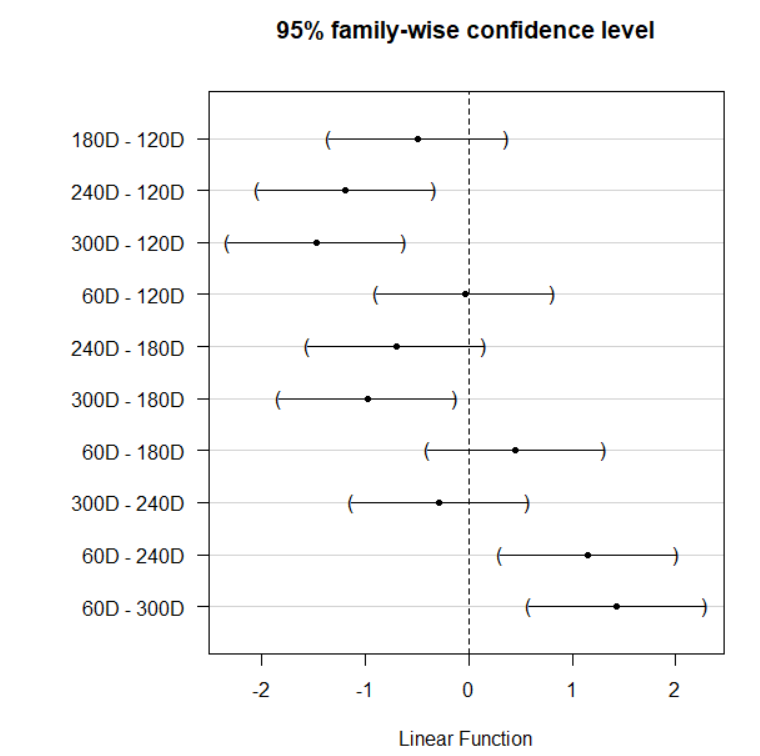
\includegraphics[width=0.6\textwidth]{image/d_信頼区間.png}
  \caption{上昇系列(D)の分散分析の結果}
  \label{fig:result_d}
\end{figure}

\section{考察}
\subsection{上昇系列と下降系列の錯視量の相違について}
図\ref{fig:60degree}より,鋏角が$60\si{\degree}$のとき,上昇系列と下降系列で錯視量に有意な差が見られ(t(12)=2.72, p=.019),図\ref{fig:group_data}より
系列Aよりも系列Dの方が錯視量が小さい.\\
図\ref{fig:120degree}より,鋏角が$120\si{\degree}$のとき,上昇系列と下降系列で錯視量に有意な差が見られない(t(12)=1.76, p=.104).\\
図\ref{fig:180degree}より,鋏角が$180\si{\degree}$のとき,上昇系列と下降系列で錯視量に有意な差が見られ(t(12)=4.17, p=.0013),図\ref{fig:group_data}より
系列Aよりも系列Dの方が錯視量が小さい.\\
図\ref{fig:240degree}より,鋏角が$240\si{\degree}$のとき,上昇系列と下降系列で錯視量に有意な差が見られ(t(12)=4.04, p=.0016),図\ref{fig:group_data}より
系列Dよりも系列Aの方が錯視量が小さい.\\
図\ref{fig:300degree}より,鋏角が$300\si{\degree}$のとき,上昇系列と下降系列で錯視量に有意な差が見られない(t(12)=0.75, p=.47).

これらの結果から,鋏角が$0-180\si{\degree}$のとき,上昇系列よりも下降系列の方が精度よく測定でき,鋏角が$180-360\si{\degree}$のとき,下降系列よりも上昇系列の方が精度よく測定できると考えられる.

\subsection{矢羽の角度と錯視量の関係について}
上昇系列における一元配置分散分析の結果(図\ref{fig:about_A_oneway}),5つの刺激条件間の錯視量の差は有意であった(F(4, 60) = 10.44, p<.001).Turkeyの多重比較の結果(図\ref{fig:about_A_multi}),
鋏角$60\si{\degree}$と$300\si{\degree}$,鋏角$120\si{\degree}$と$300\si{\degree}$,
鋏角$180\si{\degree}$と$300\si{\degree}$,鋏角$240\si{\degree}$と$300\si{\degree}$の間に有意差が見られた.

また,下降系列におけるおける一元配置分散分析の結果(図\ref{fig:about_D_oneway}),5つの刺激条件間の錯視量の差は有意であった(F(4, 60) = 10.44, p<.001).Turkeyの多重比較の結果(図\ref{fig:about_D_multi}),
鋏角$60\si{\degree}$と$240\si{\degree}$,鋏角$60\si{\degree}$と$300\si{\degree}$,
鋏角$120\si{\degree}$と$240\si{\degree}$,鋏角$120\si{\degree}$と$300\si{\degree}$の間に有意差が見られた.

したがって,どちらの系列においても,鋏角が$0-180\si{\degree}$のときは短めに錯視してしまい,鋏角が$180-360\si{\degree}$のときは長めに錯視してしまうことが分かった.

\begin{thebibliography}{9}
  \item 西崎友規子.プロジェクト実習Ⅰ ヒューマンインターフェース 実験テキスト.京都工芸繊維大学,2024年
\end{thebibliography}

\end{document}